% \documentclass{article}
% \usepackage{tikz}
% \usetikzlibrary{trees, positioning}
% \begin{document}

% \begin{figure}[h]
%     \centering
    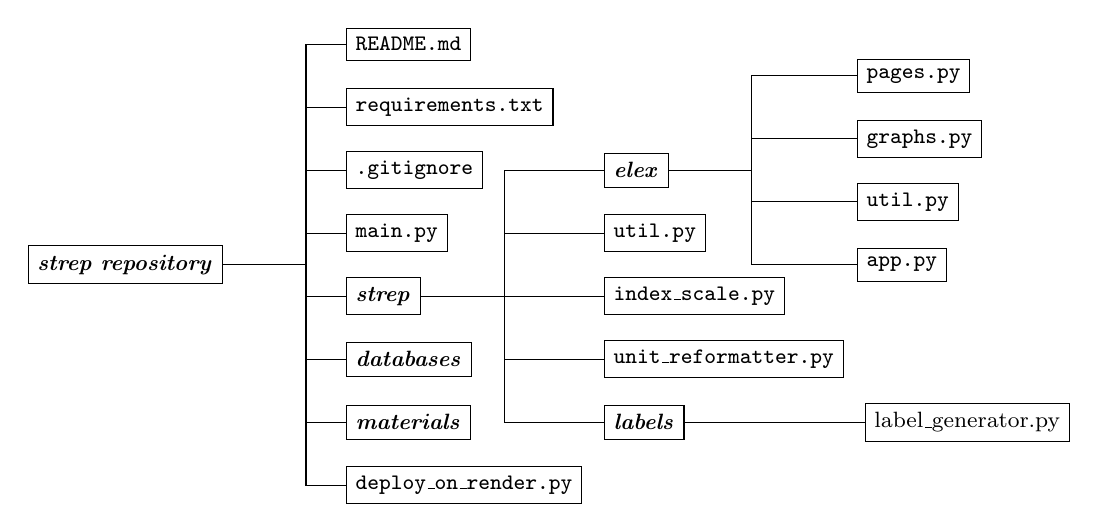
\begin{tikzpicture}[
        edge from parent path={(\tikzparentnode.east) -- +(30pt,0) |- (\tikzchildnode.west)},
        sibling distance=8mm,
        level distance=28mm,
        grow=right]
        
        \tikzstyle{every node}=[font=\footnotesize, draw, rectangle, anchor=west]
        
        \node {\emph{\textbf{strep repository}}}
        child { node {\texttt{deploy\_on\_render.py}} }
        child { node {\emph{\textbf{materials}}} }
        child { node {\emph{\textbf{databases}}} }
        child { node {\emph{\textbf{strep}}}
            child { node {\emph{\textbf{labels}}}
                child { node {label\_generator.py} }
            }
            child { node {\texttt{unit\_reformatter.py}} }
            child { node {\texttt{index\_scale.py}} }
            child { node {\texttt{util.py}} }
            child { node {\emph{\textbf{elex}}}
                child { node {\texttt{app.py}} }
                child { node {\texttt{util.py}} }
                child { node {\texttt{graphs.py}} }
                child { node {\texttt{pages.py}} }
            }
        }
        child { node {\texttt{main.py}} }
        child { node {\texttt{.gitignore}} }
        child { node {\texttt{requirements.txt}} }
        child { node {\texttt{README.md}} };
        % \node {databases}
        % child { node {xpcr} }
        % child { node {metaqure} }
        % child { node {imagenet\_classification} }
        % child { node {edge\_acc} }
        % child { node {paperswithcode} }
        % child { node {robustbench} };
    \end{tikzpicture}
%     \caption{Schematic directory structure of the strep repository (Horizontal Layout)}
% \end{figure}

% \end{document}